\documentclass{article}

% Language setting
% Replace `english' with e.g. `spanish' to change the document language
\usepackage[english]{babel}
\usepackage{float}
\usepackage{tabularx}
\usepackage{parskip} 

% Set page size and margins
% Replace `letterpaper' with`a4paper' for UK/EU standard size
\usepackage[letterpaper,top=2cm,bottom=2cm,left=3cm,right=3cm,marginparwidth=1.75cm]{geometry}

% Useful packages
\usepackage{amsmath}
\usepackage{graphicx}
\usepackage[colorlinks=true, allcolors=blue]{hyperref}

\title{DevOps report}
\author{Write names here}

\begin{document}
\maketitle

%Checklist/skeleton: https://github.com/itu-devops/lecture_notes/blob/master/REPORT.md
% revised idea for skeleton:
\section{System's Perspective}
\subsection{Design of the system} [ALL, intially JACOB AND FREDERIK]
\subsection{Architecture of the system} ALL, initially ALBERT AND RASMUS]
\subsection{Dependencies} [ALEKXANDER AND JACOB] \\
\subsubsection{Software dependencies}
%skal vi lave en rigtig dep. graph? (med pile osv)
The dependencies of the system is derived via GitHub from the \texttt{mvc-minitwit.csproj} 
and 

\texttt{HomeControllerTests.csproj} project files. These correspond to the MiniTwit and testing project respectively. The dependency graph can be found on \url{https://github.com/albertbethlowsky/DevOpsGroupH/network/dependencies}. A small snippet of the current graph for both projects can be seen below:
\begin{figure}[H]
\centering
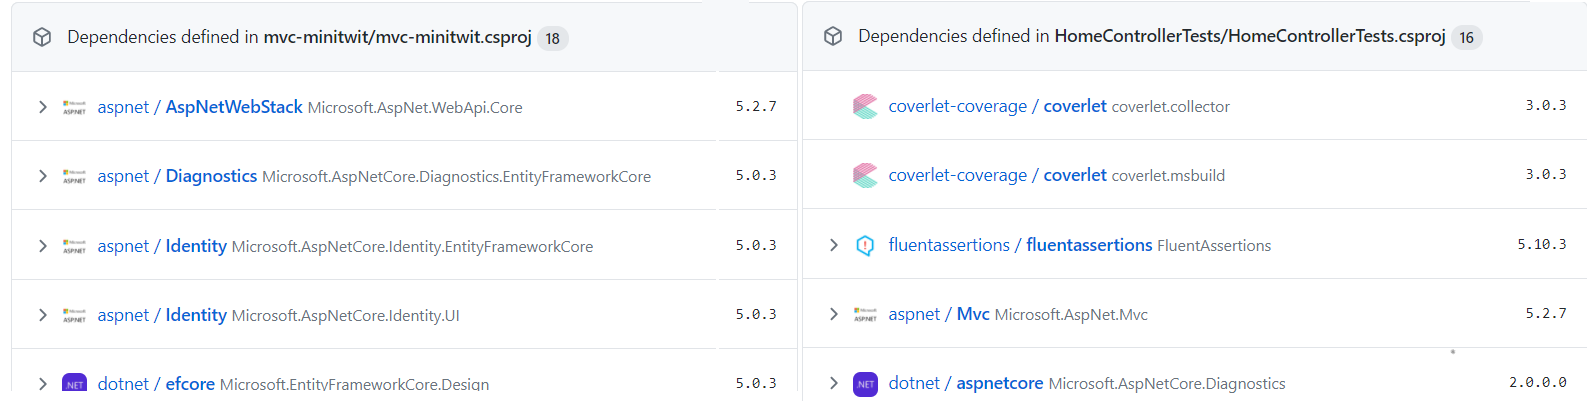
\includegraphics[width=1.1\textwidth]{images/dependencies-snip.png}
\caption{\label{fig:dep1}Snippet of dependency graphs of both \texttt{mvc-minitwit.csproj} and \\\\ \texttt{HomeControllerTests.csproj}}
\end{figure}
\subsubsection{Cloud dependencies}
These dependencies are related to the services hosted on Azure, where MiniTwit also is deployed. 

\begin{table}[H]
\begin{tabularx}{\textwidth}{|l|l|l|X|}
\hline
    \textbf{Name} & \textbf{Service} & \textbf{Provider} & \textbf{Description} \\ \hline
    neutrals-minitwit & App Service & Microsoft Azure & Hosting of web applications (.NET application) \\ \hline
    minitwit-neutrals & App Service & Microsoft Azure & Hosting of web applications (prometheus, grafana) \\ \hline
    neutralsseq & App Service & Microsoft Azure & Hosting of web applications (Datalust - Seq) \\ \hline
    minitwit-neutrals & SQL Server & Microsoft Azure & Hosting of SQL database \\ \hline
    minitwitDb (minitwit-neutrals) & SQL database & Microsoft Azure & SQL database \\ \hline
    neutralsminitwit.azurecr.io & Docker container & Azure Container Registry & Containerizing of applications \\ \hline
\end{tabularx}
\end{table}

\subsubsection{Important interactions of subsystems} [FREDERIK, JACOB, ALEKXANDER]
%how does components talk together.. e.g. Sequence diagrams
\subsection{Current state of the system} 
[ALEKXANDER AND FREDERIK]
With the help of different static analysis tools, it's possible to get a sense of the state of the system, including an estimation of the technical debt. Their respective results are briefly presented:

\subsubsection*{SonarCloud}
Based on the results from SonarCloud the systems seems to be in a satisfactory state, however there are a few caveats to point out. The auto-generated contents of \texttt{Migrations/}, and the \texttt{wwwroot/lib} folder has been excluded from all analysis since the latter contains deprecated jQuery libraries. These were given from the beginning, and were thus deemed out of scope to fix with time available. 

\begin{figure}[H]
\centering
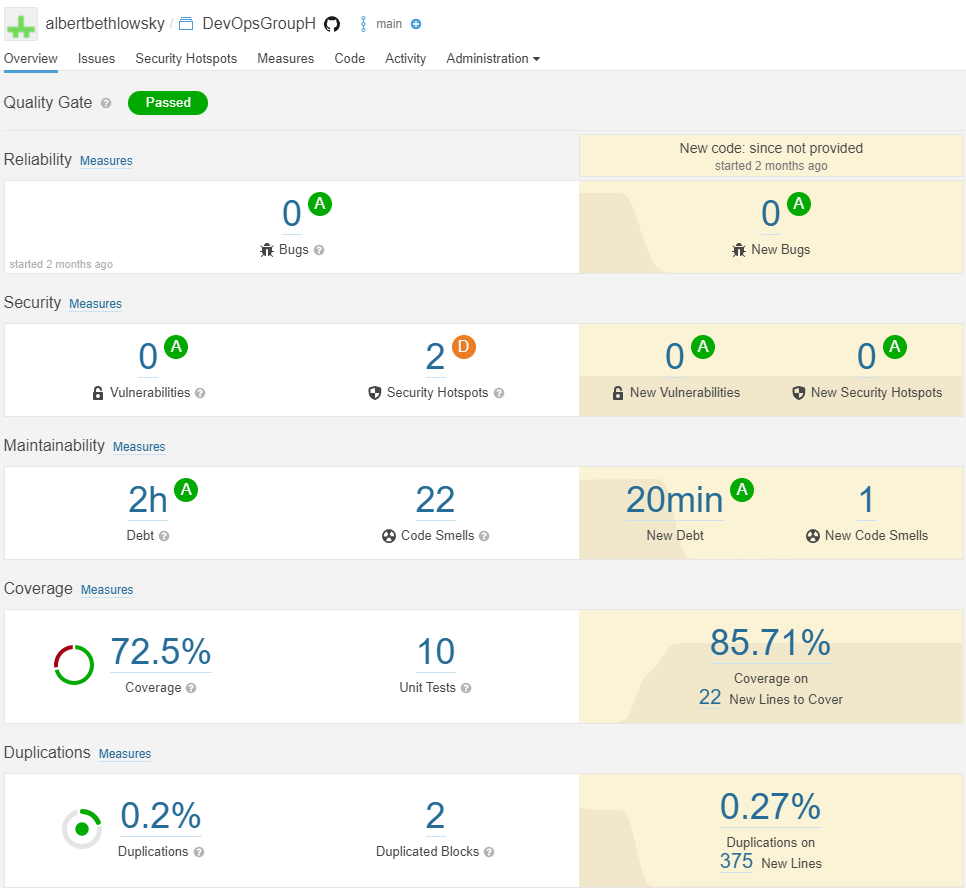
\includegraphics[width=0.7\textwidth]{images/sonarcloud.png}
\caption{\label{fig:dep1} Results from SonarCloud and its different categories, with the Quality Gate passed}
\end{figure}

The boiler plate, initialization files \texttt{Program.cs}, \texttt{Startup.cs} are excluded from test coverage analysis. \texttt{HomeController.cs} is also excluded from test coverage due to project scope and challenges with mocking cookies.
% her antages at læser ved hvad HomeController.cs er
From the maintainability category, there's "2 hours" of debt, but it's worth mentioning that it's a relative estimate based on "Code smells", uncovered and duplicated lines. This estimate should be compared with the estimates from the other tools.   
\subsubsection*{Code Climate}
The repository has a maintainability grade of "B", which with their estimates would be about 2 days of technical debt. There are 19 issues in total, split into 8 of duplication and 11 code smells. The file with the lowest maintainability score is \texttt{HomeController.cs} and has a "C", which would be the file to prioritize first for refactoring. The same files and folders have been excluded as with SonarCloud. %check this

As a side note a big source of the issues in both \texttt{HomeController.cs} and \texttt{APIController.cs} comes in the shape of \textit{"Avoid too many return statements"}. This is an issue that can be taken with a grain of salt, since it relates to the debate of "clean OOP" approach, which is harder to implement in server/API application. %let me know if u agree/disagree here  


\begin{figure}[H]
\centering
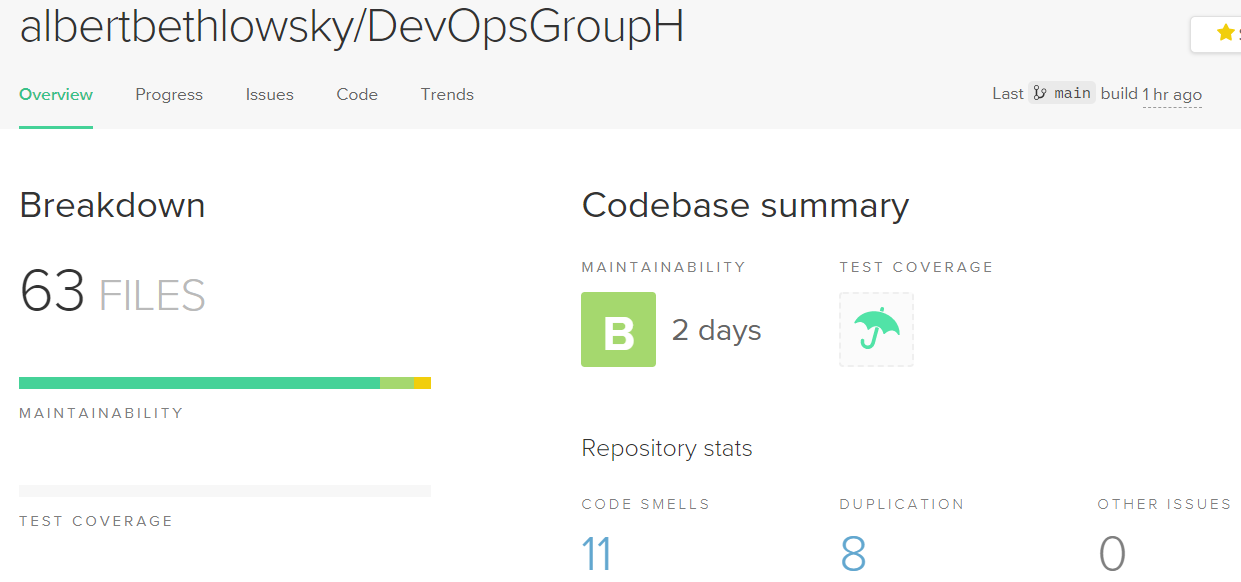
\includegraphics[width=0.7\textwidth]{images/codeclimate.png}
\caption{\label{fig:dep1} Code Climate summary and overview}
\end{figure}

\subsubsection*{Better Code}
[Albert]

\subsubsection*{InferSharp}



At the top of the \texttt{README.md}, badges of the different tools have been added to help give a quick overview of their results. It's worth mentioning that technical debt is a relative term, and as seen between the tools, can vary quite a lot (e.g. 2 days to 2 hours).

\subsection{Licenses and compatibility}[ALBERT AND RASMUS]

\section{Process perspective}
\subsection{Interactions between developers} [RASMUS & ALBERT]
\subsection{Team organization} [RASMUS & ALBERT]
\subsection{Description of CI/CD pipelines, stages and tools}[ALEKXANDER & FREDERIK]
Azure DevOps is used to manage the CI/CD pipelines for the project. See azure-pipelines.yml for the stages and tools utilized in our pipeline. Terraform will be applied to the pipeline in future iterations such that we have automated the infrastructure (IaC) maintenance.  

\subsection{Repository arrangement/organization}[FREDERIK & JACOB]
\subsection{Applied Branching Strategy}[ALEXANDER & FREDERIK] 
Throughout the project a "Long-Running Branches" strategy has been used. The \textit{master} branch has primarily been used for code releases or \texttt{.yml} pipeline changes. The  \textit{development} branch was used to merge all the features back into, so that it in turn becomes can be merged into \textit{master} as the next stable release. Finally the individual feature branches correspond to the issues on the Task board on GitHub. Each feature branch is named after their issue number, e.g. \texttt{fea#34APIController}. Pull requests to merge the branches has been used, but not with absolute consistency.   
\subsection{Applied development process and related tools}[JACOB & FREDERIK]
\subsubsection{Simple Kanban board}[FREDERIK & RASMUS]
We have utilized github's projects to manage our tasks. The board consists of the traditional kanban setup with 'tasks', 'in progress', 'parked', and 'done'. 
\subsection{Monitoring}[JACOB & ALEKXANDER]
% it's hard to tell exactly what they measure..
\begin{figure}[H]
\centering
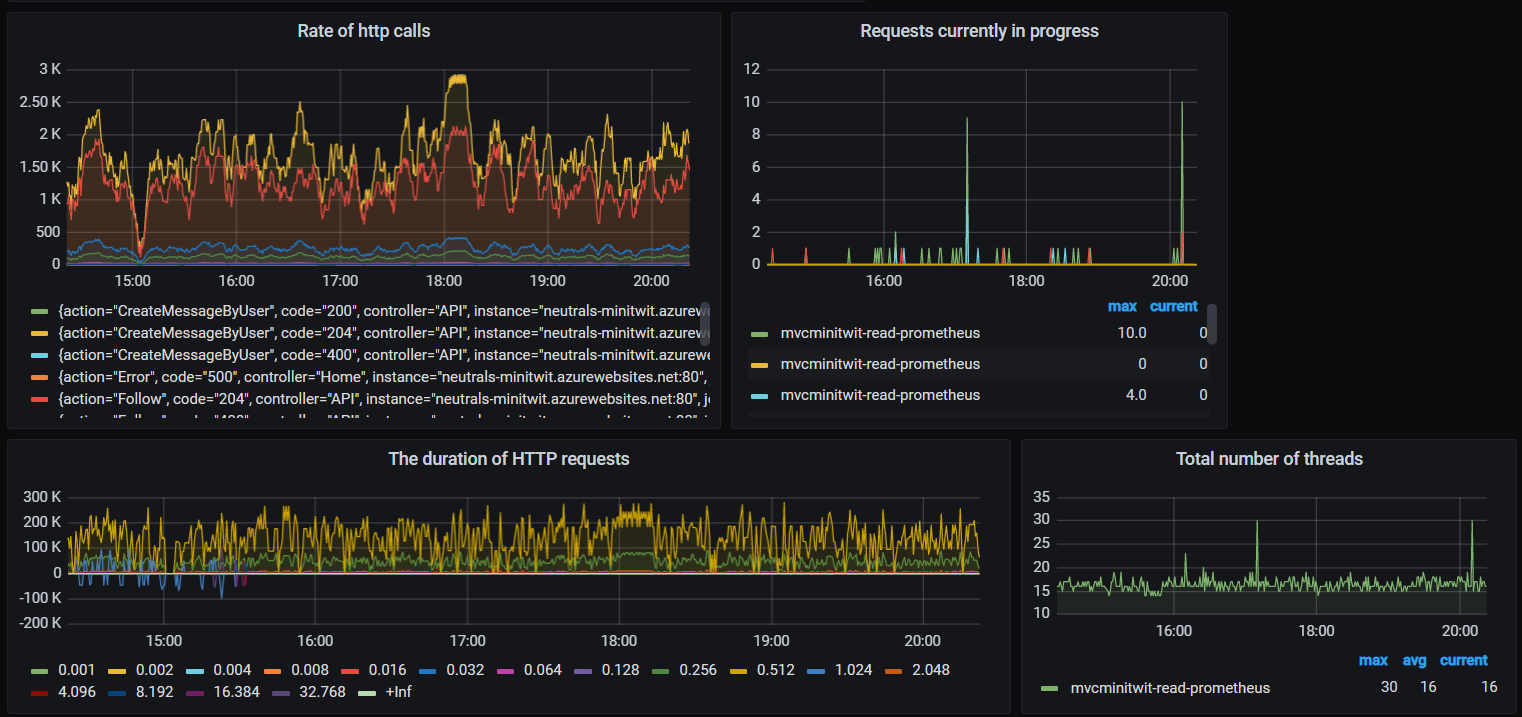
\includegraphics[width=1\textwidth]{images/dashboard.png}
\caption{\label{fig:dashboard} Grafana dashboards}
\end{figure}
\subsection{Logging and log aggregation} [JACOB & ALEKXANDER]
\subsection{Brief security assessment} [RASMUS & ALBERT]
\subsection{Applied scaling and load balancing strategy} [FREDERIK AND ALEKXANDER]
Due to different challenges with Azure Kubernetes Service on Azure and Azure DevOps it was not possible to implement scaling within the given time frame. We did however implement azure's 'scale out' service which is a built-in feature that helps applications perform their best when demand changes.  %hvor skal man uddybe grundene?    

\section{Lessons learned perspective}
\subsection{Evolution and refactoring} [ALL, init JACOB AND RASMUS]
\subsection{Operation} [ALL, init ALEKXANDER AND ALBERT]
\subsection{Maintenance} ALL, init FREDERIK and JACOB]



\bibliographystyle{alpha}
\bibliography{sample}

\end{document}